%!TEX root = karen.tex

\chapter{Parallel Solvers}
\label{sec:rbffd_gpu}


Solving PDEs in a distributed computing environment requires three design decisions \cite{Saad2003}. First, the domain is partitioned and distributed across compute nodes in some fashion. Intelligent partitioning impacts load balancing on processors to minimize computation to communication ratio; imbalanced computation across processors can cause excessive delay per iteration as processors wait to receive information. Second, one must decide what information each processor is able to access regarding node information, solution values, etc and establish index mappings that translate between a processor's local context and the global problem. In situations where processors are not aware of all nodes/solution values in the global domain, the index mappings are essential to maintaining solution consistency at each time-step. Last but not least, each processor can re-order nodes locally in an effort to improve solver efficiency and local system conditioning. Node ordering also allows us to minimize data transfer between CPU and GPU. 


Parallelization of the RBF-FD method is achieved at two levels. First, the physical domain of the problem---in this case, the unit sphere---is partitioned into overlapping subdomains, each handled by a different CPU process. All CPUs operate independently to compute/load RBF-FD stencil weights, run diagnostic tests and perform other initialization tasks. A CPU computes only weights corresponding to stencils centered in the interior of its partition. After initialization, CPUs continue concurrently to solve the PDE. Communication barriers ensure that the CPUs execute in lockstep to maintain consistent solution values in regions where partitions overlap. 
The second level of parallelization offloads time-stepping of the PDE to the GPU.
Evaluation of the right hand side of Equation~(\ref{eq:evaluation_with_hyperviscosity}) is data-parallel: the solution derivative at each stencil center is evaluated independently of the other stencils. This maps well to the GPU, offering decent speedup even in unoptimized kernels. Although the stencil weight calculation is also data-parallel, we assume that in this context that the  weights are precomputed and loaded once from disk during the initialization phase. 


\section{Paritioning}

We partition the domain assuming that domains overlap. Processor views of the domain are limited to only nodes required by stencils under processor control. Subset of the grid. Subset of the stencils. 

Preliminary decomposition is slicing horizontally in the domain. 

Load balancing important and can be handled by METIS.

\section{Global and local index maps}
Due to the local view of each processor, local index maps are much shorter than global maps. They run from 0 to $N_{p}$. 

STL Maps based

\section{Local node ordering}

The local index set is ordered as ${QmB, BmO, O, R}$ 

Domain boundary nodes appear at beginning of the list 

\section{Two level parallelism}

Our current implementation assumes that we are computing on a cluster of CPUs, with one GPU attached to each CPU. The CPU maintains control of execution and launches kernels on the GPU that execute in parallel. Under the OpenCL standard \cite{OpenCL2009}, a tiered memory hierarchy is available on the GPU with \textit{global device memory} as the primary and most abundant memory space. The memory space for GPU kernels is separate from the memory available to a CPU, so data must be explicitly copied to/from global device memory on the GPU. 


\section{Distributed Solvers}
Need partitioning, global and local index maps, and local ordering for a distributed \cite{Saad2003} 

\subsection{Node Partitioning}

Figure~\ref{fig:decomposed_sphere} illustrates a partitioning of $N=10,201$ nodes on the unit sphere onto four CPUs. Each partition, illustrated as a unique color, represents set $\setAllNodes$ for a single CPU. 
Alternating representations between node points and interpolated surfaces illustrates the overlap regions where nodes in sets $\mathcal{O}$ and $\mathcal{R}$ (i.e., nodes requiring MPI communication) reside. As stencil size increases, the width of the overlap regions relative to total number of nodes on the sphere also increases. 
\authnote{Q: what is the percentage overlap for $n$? $\frac{1}{2} n^{\frac{1}{d}}$ gives depth into neighbor since n is uniformly sampled we expect a cube shape. (SHould be literature on this...no?)} % assume sphere, sqrt of N for scaling area covered by stencil}

The linear partitioning in Figure~\ref{fig:decomposed_sphere} was chosen for ease of implementation. Communication is limited for each
processor to left and right neighbors only, which simplifies parallel debugging. This partitioning, however, does not guarantee properly balanced computational work-loads. Other partitionings of the sphere exist but are not studied here because this paper's focus is neither on efficiency nor on selecting a partitioning strategy for maximum accuracy. Examples of alternative approaches include a cubed-sphere \cite{Ivan2011} or icosahedral geodesic grid \cite{Randall2002}, which can evenly balance the computational load across partitions. Other interesting partitionings can be generated with software libraries such as the METIS \cite{Karypis1999} family of algorithms, capable of partitioning and reordering directed graphs produced by RBF-FD stencils. 

\begin{figure}[ht!]
\begin{center}
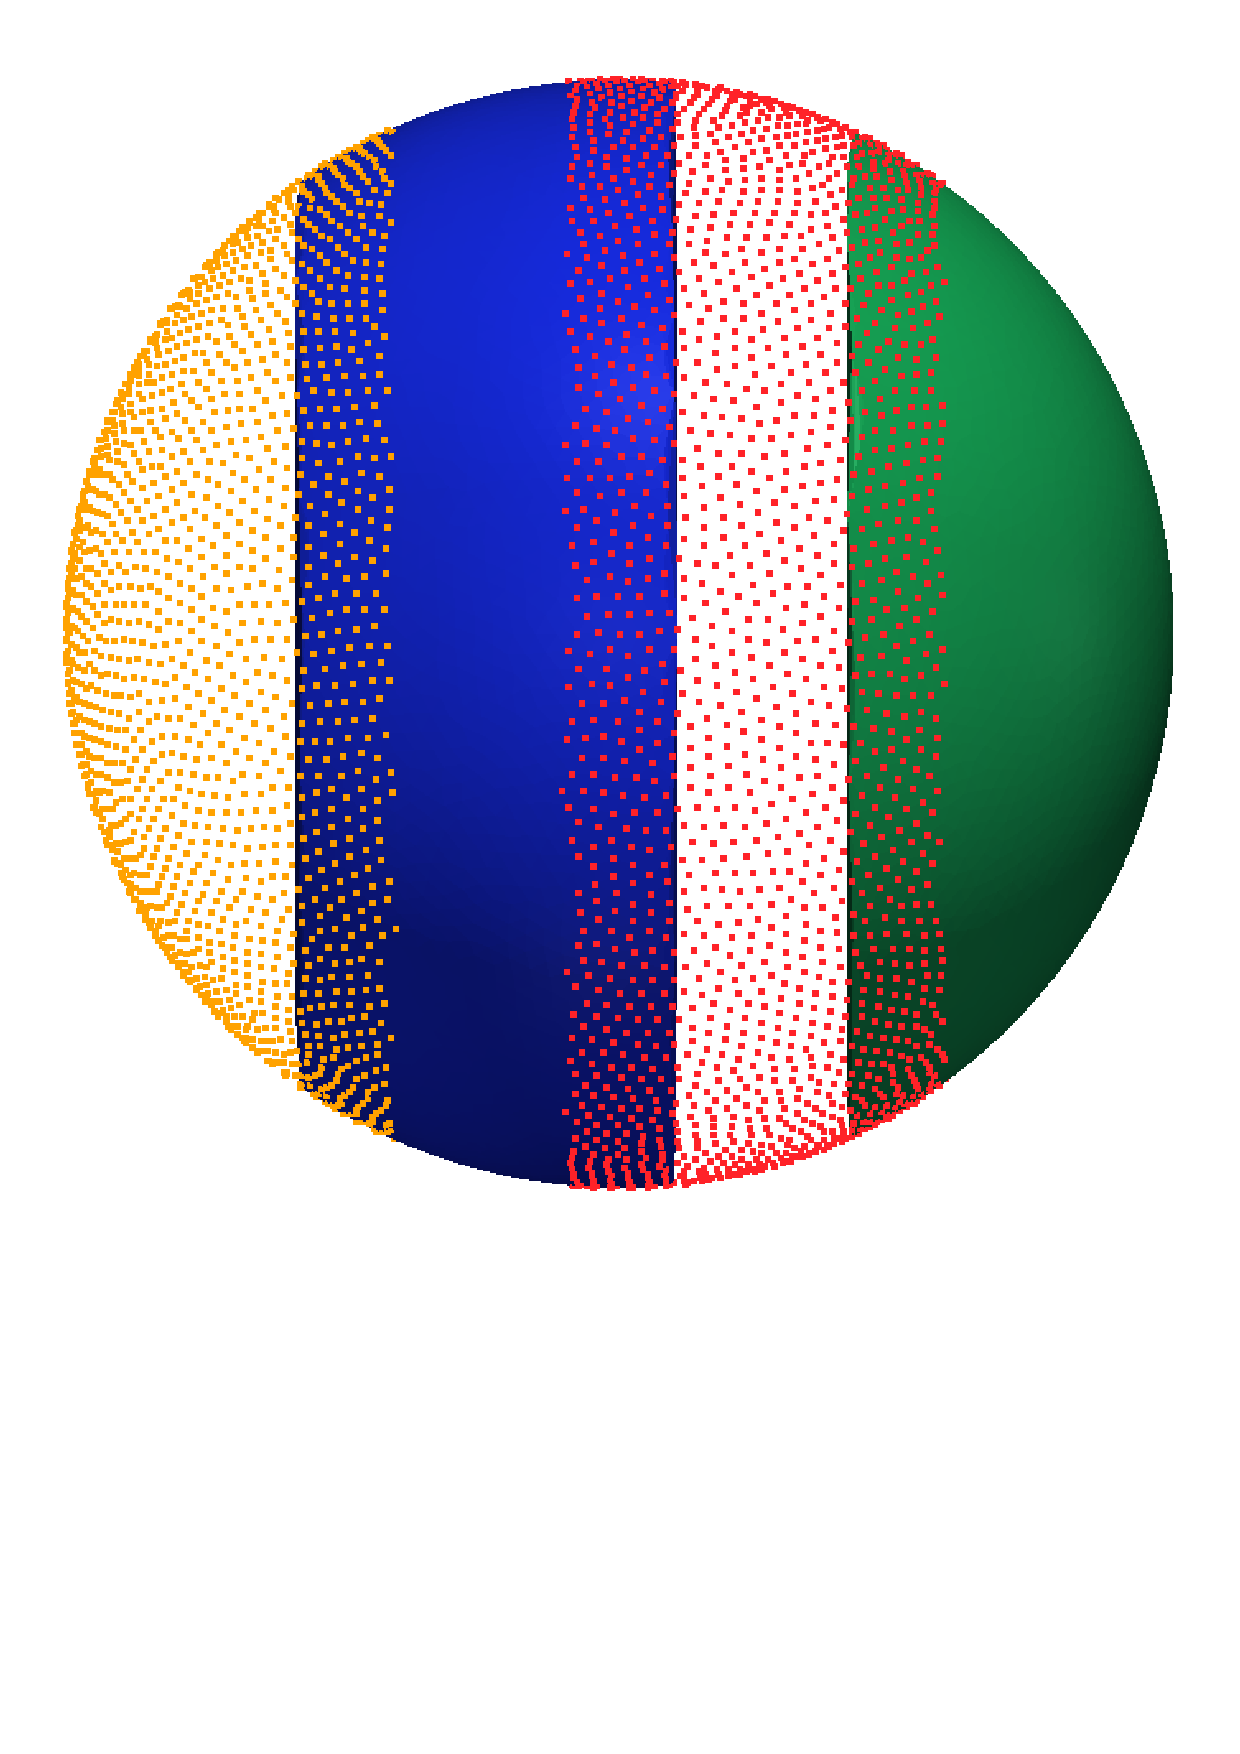
\includegraphics[width=2.5in]{figures/paper1/figures/vortex_rollup/4procs_N10K_n31.pdf}
\caption{Partitioning of $N=10,201$ nodes to span four processors with stencil size $n=31$.  }
\label{fig:decomposed_sphere}
\end{center}
\end{figure}

\authnote{Need to flesh detail on ParMETIS, two dimensional partitioning and case when a node value is required by multiple processors}


\subsection{Global and Local Indices}

\subsection{Local Node Ordering} 
After partitioning, each CPU/GPU is responsible for its own subset of nodes. 
To simplify accounting, we track nodes in two ways. Each node is assigned
a global index, that uniquely identifies it. This index follows the node 
and its associated data as it is shuffled between processors. In addition, 
it is important to treat the nodes on each CPU/GPU in an identical manner. 
Implementations on the GPU are more efficient when node indices
are sequential. Therefore, we also assign a local index for the nodes on 
a given CPU, which run from 1 to the maximum number of nodes on that CPU. 

It is convenient to break up the nodes on a given CPU into various sets
according to whether they are sent to other processors, are retrieved from 
other processors, are permanently on the processor, etc. Note as well, 
that each node has a home processor since the RBF nodes are partitioned into 
multiple domains without overlap.
Table~\ref{tbl:stencil_sets}, defines the collection of index lists that each CPU must maintain for both multi-CPU and multi-GPU implementations.  


Figure~{\ref{fig:stencilSets2CPU}} illustrates a configuration with two 
CPUs and two GPUs, and 9 stencils, four on CPU1, and five on CPU2, separated
by a vertical line in the figure. Each stencil
has size $n=5$. In the top part of the figures, the stencils are laid out
with blue arrows pointing to stencil neighbors and creating the edges of a directed adjacency graph. Note that the connection between two nodes is not 
always bidirectional. For example, node 6 is in the stencil of node 3, but 
node 3 {\em is not\/} a member of the stencil of node 6. 
Gray arrows point to stencil neighbors outside the small window and are not relevant to the following discussion, which focuses only on data flow between 
CPU1 and CPU2. 
Since each CPU is responsible for the derivative evaluation and solution updates for any stencil center, it is clear that some nodes have a stencil with nodes that are on a different CPU. For example, node 8 on CPU1 has a stencil comprised of
nodes 4,5,6,9, and itself. The data associated with node 6 must be retrieved
from CPU2. Similarly, the data from node 5 must be sent to CPU2 to 
complete calculations at the center of node 6.

The set of all nodes that a CPU interacts with is denoted by $\setAllNodes$, which includes not only the nodes stored on the CPU, but the nodes required from other CPUs to complete the calculations. 
The set $\setCenters\in\setAllNodes$ contains the nodes at which the CPU 
will compute derivatives and apply solution updates. 
The set $\setDepend = \setAllNodes \backslash \setCenters$ 
is formed from the set of nodes whose values must be retrieved from another CPU. 
For each CPU, the set $\setProvide\in\setCenters$ is sent to other CPUs. The set $\setBoundary\in\setCenters$ consists of nodes that depend on  values from $\setDepend$ in order to evaluate derivatives. Note that $\setProvide$ and $\setBoundary$ can overlap, but differ in size, since the directed adjacency graph produced by stencil edges is not necessarily symmetric. The set $\setBoundary \backslash \setProvide$ represents nodes that depend on $\setDepend$ but are not sent to other CPUs, while $\setCenters \backslash \setBoundary$ are nodes that have no dependency on information from other CPUs.
The middle section Figure~\ref{fig:stencilSets2CPU} lists global node indices contained in $\setAllNodes$ for each CPU. Global indices are paired with local indices to indicate the node ordering internal to each CPU. The structure of set $\setAllNodes$,
   \begin{equation}
 		\setAllNodes = \{ \mathcal{Q}\backslash\mathcal{B} \ \ \mathcal{B}\backslash\mathcal{O} \ \ \mathcal{O} \ \ \setDepend \},
            \label{eqn:decompose_g}
        \end{equation}
 is designed to simplify both CPU-CPU and CPU-GPU memory transfers by grouping nodes of similar type. The color of the global and local indices in the figure
 indicate the sets to which they belong. They are as follows: white represents $\setCenters \backslash \setBoundary$, 
 yellow represents $\setBoundary \backslash \setProvide$, green indices 
 represent $\setProvide$, and red represent $\setDepend$.  


        \begin{table}[t]
            \begin{center}
                \begin{tabular}{l l}
                    \hline
                    $\setAllNodes$ &: all nodes received and contained on the CPU/GPU $g$ \\
                    $\setCenters$ &: stencil centers managed by $g$ 
					(equivalently, stencils computed by $g$) \\
                    $\setBoundary$ &: stencil centers managed by $g$ that
                    require nodes from another CPU/GPU \\
                    $\setProvide$ &: nodes managed by $g$ that are sent to other CPUs/GPUs  \\
                    $\setDepend$ &: nodes required by $g$ that are managed by another CPU/GPU \\
                    \hline
                \end{tabular}
                \caption{Sets defined for stencil distribution to multiple CPUs}
                            \label{tbl:stencil_sets}
            \end{center}
        \end{table}

        \begin{figure}[ht] 
            \centering
            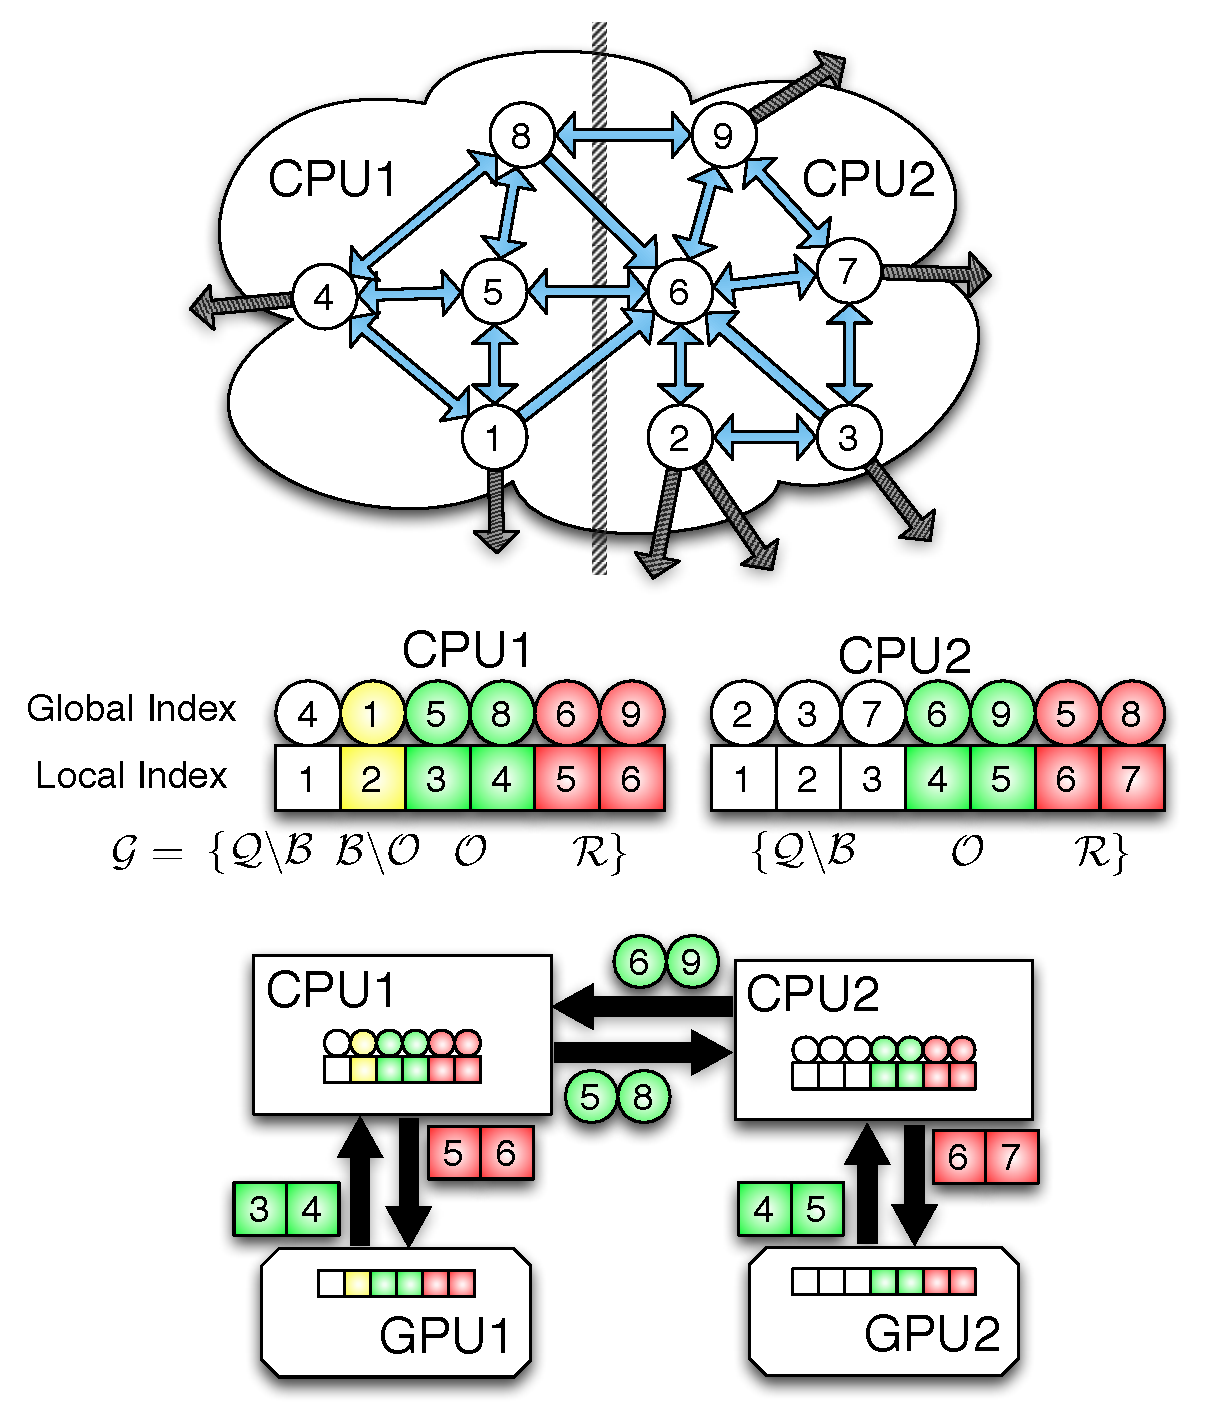
\includegraphics[width=3.5in]{figures/paper1/figures/omnigraffle/SimpleExample.pdf} 
            \caption{Partitioning, index mappings and memory transfers for nine stencils ($n=5$) spanning two CPUs and two GPUs. Top: the directed graph created by stencil edges is partitioned for two CPUs. Middle: the partitioned stencil centers are reordered locally by each CPU to keep values sent to/received from other CPUs contiguous in memory. Bottom: to synchronize GPUs, CPUs must act as intermediaries for communication and global to local index translation. Middle and Bottom: color coding on indices indicates membership in sets from Table~\ref{tbl:stencil_sets}: $\setCenters \backslash \setBoundary$ is white, $\setBoundary \backslash \setProvide$ is yellow, $\setProvide$ is green and $\setDepend$ is red.
            }
            \label{fig:stencilSets2CPU}
        \end{figure}	

   
 The structure of $\setAllNodes$ offers two benefits: first, solution values in $\setDepend$ and $\setProvide$ are contiguous in memory and can be copied to or from the GPU without the filtering and/or re-ordering normally required in preparation for efficient data transfers. Second, asynchronous communication allows for the overlap of communication and computation. This will be considered as part of future research on algorithm optimization.  Distinguishing the set $\mathcal{B} \backslash \mathcal{O}$ allows the computation of $\mathcal{Q}\backslash \mathcal{B}$ while waiting on $\mathcal{R}$. 



When targeting the GPU, communication of solution or intermediate values is a four step process:
        \begin{enumerate}
    \item Transfer $\mathcal{O}$ from GPU to CPU
	\item Distribute $\mathcal{O}$ to other CPUs, receive $R$ from other CPUs
	\item Transfer $\mathcal{R}$ to the GPU
	\item Launch a GPU kernel to operate on $\mathcal{Q}$
     \end{enumerate} 
The data transfers involved in this process are illustrated at the bottom of Figure~\ref{fig:stencilSets2CPU}.
    Each GPU operates on the local indices ordered 
according to Equation~(\ref{eqn:decompose_g}). The set 
$\setProvide$ is copied off the GPU and into CPU memory as one contiguous memory block. The CPU then maps local to global indices and transfers $\setProvide$ to other CPUs. CPUs send only the subset of node values from $\setProvide$ that is required by the destination processors, but it is important to note that node information might be sent to several destinations. 
As the set $\setDepend$ is received, the CPU converts back from global to local indices before copying a contiguous block of memory to the GPU. 

        This approach is scalable to a very large number of 
		processors, since the individual processors do not require the 
		full mapping between RBF nodes and CPUs. 


\section{Overlapping Computation and Communication} 
Need to describe our approach to launch 

In simplest form (\& indicates an overlapped execution; overlapping is possible by non-blocking launches to the GPU before comm is started): 
\begin{itemize} 
\item $ U_{Q \backslash B}' = A_{Q \backslash B} U_{Q \backslash B}$ 
\item \& MPI\_alltoallv
\item $ U_{B}' = A_{B} U_{B}$ 
\end{itemize} 
This form benefits because stencils are operated on in their entirety. For the GPU this is important because we maintain SIMD nature. 

A more complex form which might overlap more comm and comp depending on the size of B (i.e., might be beneficial for large stencil sizes): 
\begin{itemize} 
\item $ U_{Q \backslash B}' = A_{Q \backslash B} U_{Q \backslash B}$ 
\item \& MPI\_alltoallv
\item \& $ U_{B}' = A_{B \backslash R} U_{B \backslash R}$  (partial sparse vector product)
\item $ U_{B}' += A_{R} U_{R}$ 
\end{itemize} 

Note that there is no non-blocking version of MPI\_alltoallv within the MPI standard, so the above two algorithms will not be overlapped when computing on the CPU. To overlap on the CPU, \cite{Kandalla2011} refers to the non-blocking collective as MPI\_ialltoallv. With a collective like this, we could enforce a pattern like: 
\begin{itemize} 
\item MPI\_alltoallv
\item \& $ U_{Q \backslash B}' = A_{Q \backslash B} U_{Q \backslash B}$ 
\item \& $ U_{B}' = A_{B \backslash R} U_{B \backslash R}$  (partial sparse vector product)
\item MPI\_wait
\item $ U_{B}' += A_{R} U_{R}$ 
\end{itemize} 

%K. Kandalla, H. Subramoni, K. Tomko, D. Pekurovsky, S. Sur and D.K. Panda, "High-performance and scalable non-blocking all-to-all with collective offload on InfiniBand clusters: a study with parallel 3D FFT", Computer Science - Research and Development, vol. 26(3-4):237-246, 2011.
%T. Hoefler, A. Lumsdaine and W. Rehm, "Implementation and Performance Analysis of Non-Blocking Collective Operations for MPI", International Conference for High Performance Computing, Networking, Storage and Analysis (SC07), Reno, USA, 2007.

\section{Targeting the GPU}

\authnote{The basic primitives necessary to parallelize our problems: SpMV, AXPY and }

\subsection{Explicit Solvers}


Our implementation leverages the GPU for acceleration of the standard fourth order Runge-Kutta (RK4) scheme. Nodes are stationary, so stencil weights are calculated once at the beginning of the simulation, and reused in every iteration. To avoid the cost of calculating stencil weights each time a test case is run, they are written to disk and loaded from file on subsequent runs. There is one set of weights computed for each new grid.  Ignoring code initialization, the cost of the algorithm is simply the explicit time advancement of the solution. 

\begin{figure}[t]
      \centering
       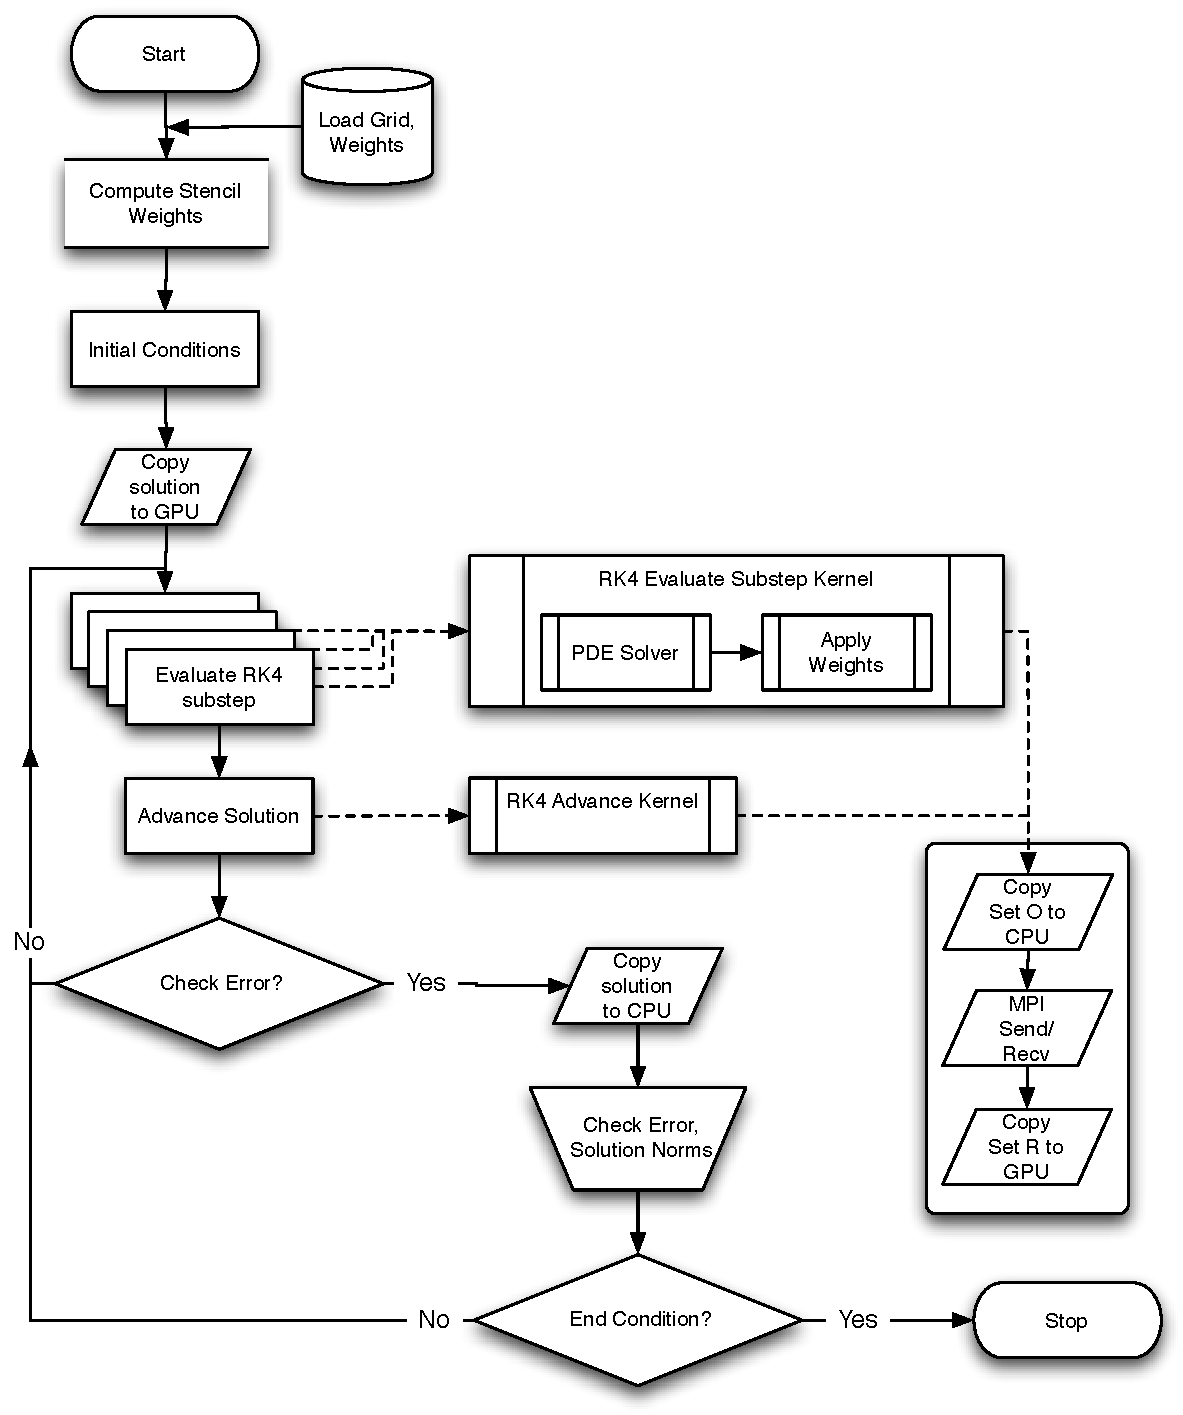
\includegraphics[width=5in]{figures/paper1/figures/omnigraffle/RK4_multi_GPU_flow.pdf}
      \caption{Workflow for RK4 on multiple GPUs. }
      \label{fig:multi_GPU_flow}
\end{figure}

Figure~\ref{fig:multi_GPU_flow} summarizes the time advancement steps for the multi-CPU/GPU implementation. The RK4 steps are: 
\begin{eqnarray*} 
\mathbf{k}_1 &=& \Delta t f(t_n, \mathbf{u}_n) \\
\mathbf{k}_2 &=& \Delta t f(t_n+\frac{1}{2}\Delta t, \mathbf{u}_n + \frac{1}{2}\mathbf{k}_1) \\
\mathbf{k}_3 &=& \Delta t f(t_n+\frac{1}{2}\Delta t, \mathbf{u}_n + \frac{1}{2}\mathbf{k}_2) \\
\mathbf{k}_4 &=& \Delta t f(t_n+\Delta t, \mathbf{u}_n + \mathbf{k}_3) \\
\mathbf{u}_{n+1} &=& \mathbf{u}_{n} + \frac{1}{6}(\mathbf{k}_1 + 2\mathbf{k}_2 + 2\mathbf{k}_3 +\mathbf{k}_4),
\label{eqn:rk4}
\end{eqnarray*}
where each equation has a corresponding kernel launch. To handle a variety of Runga-Kutta implementations, steps $\mathbf{k}_{1\rightarrow4}$ correspond to calls to the same kernel with different arguments. The evaluation kernel returns two output vectors: 
\begin{enumerate} 
\item $\mathbf{k}_i = \Delta t f(t_n + \alpha_{i} \Delta t, \mathbf{u}_n + \alpha_{i} \mathbf{k}_{i-1})$, for steps $i=1,2,3,4$, and
\item  $\mathbf{u}_n + \alpha_{i+1} \mathbf{k}_i$
\end{enumerate} 
We choose $\alpha_{i}=0, \frac{1}{2}, \frac{1}{2}, 1, 0$ and $\mathbf{k}_{0} = \mathbf{u}_n$. The second output for each $\mathbf{k}_{i=1,2,3}$ serves as input to the next evaluation, $\mathbf{k}_{i+1}$. In an effort to avoid an extra kernel launch---and corresponding memory loads---the SAXPY that produces the second output uses the same evaluation kernel. Both outputs are stored in global device memory. When the computation spans multiple GPUs, steps $\mathbf{k}_{1\rightarrow3}$ are each followed by a communication barrier to synchronize the subsets $\mathcal{O}$ and $\mathcal{R}$ of the second output (this includes copying the subsets between GPU and CPU). An additional synchronization occurs on the updated  solution, $\mathbf{u}_{n+1}$, to ensure that all GPUs share a consistent view of the solution going into the next time-step.

To evaluate $\mathbf{k}_{1\rightarrow4}$, the discretized operators from Equation~(\ref{eq:evaluation_with_hyperviscosity}) are applied using sparse matrix-vector multiplication. If the operator $D$ is composed of multiple derivatives, a differentiation matrix for each derivative is applied independently, including an additional multiplication for the discretized $H$ operator.
 On the GPU, the kernel parallelizes across rows of the DMs, so all derivatives for stencils are computed in one kernel call.


For the GPU, the OpenCL language \cite{OpenCL2009} assumes a lowest common denominator of hardware capabilities to provide functional portability. For example, all target architectures are assumed to support some level of SIMD (Single Instruction Multiple Data) execution for kernels. Multiple \textit{work-items} execute a kernel in parallel. 
A collection of work-items performing the same task is called a \textit{work-group}. While a user might think of work-groups as executing all work-items simultaneously, the work-items are divided at the hardware level into one or more SIMD \textit{warps}, which are executed by a single multiprocessor. On the family of Fermi GPUs, a warp is 32 work-items \cite{CudaGuide2011}. 
OpenCL assumes a tiered memory hierarchy that provides fast but small \textit{local memory} space that is shared within a work-group \cite{OpenCL2009}. Local memory on Fermi GPUs is 48 KB per multiprocessor \cite{CudaGuide2011}. The \textit{global device memory} allows sharing between work-groups and is the slowest but most abundant memory. 
In the GPU computing literature, the terms \textit{thread} and \textit{shared memory} are synonymous to \textit{work-item} and \textit{local memory} respectively, and are preferred below. 

Although the primary focus of this paper is the implementation 
and verification of the RBF-FD method across multiple CPUs and GPUs, 
we have nonetheless tested two approaches to the computation of derivatives 
on the GPU to 
assess the potential for further improvements in performance. 
In both cases, the stencil weights are stored in CSR format \cite{Bell2009}, 
a packed one-dimensional array in global memory with all the weights 
of a single stencil in consecutive memory addresses. Each operator is stored as an independent CSR matrix. The consecutive ordering on the weights implies that the solution vector, structured according to the ordering of set $\mathcal{G}$ is treated as random access. 

All the computation on the GPU is performed in 8-byte double precision. 


\subsubsection{Naive Approach: One thread per stencil}

In this first implementation, each thread computes 
the derivative at one stencil center  (Figure~\ref{fig:oneThreadPerStencil}). 
The advantage of this approach is trivial concurrency.  Since each stencil has the same number of neighbors, each derivative has an identical number of computations. As long as the number of stencils is a multiple of the warp size, there are no idle threads. Should the total number of stencils be less than a multiple of the warp size, the final warp would contain idle threads, but the impact on efficiency would be minimal assuming the stencil size is sufficiently large. 

Perfect concurrency from a logical point of view does not 
imply perfect efficiency in practice. 
Unfortunately, the naive approach 
is memory bound. When threads access weights in global memory, 
a full warp accesses a 128-byte segment in a single memory operation \cite{CudaGuide2011}.
Since each thread handles a single stencil, the various threads in a warp access data in very disparate areas of global memory, rather than the same segment. This leads to very large slowdowns as extra memory operations are added for each 128-byte segment that the threads of a warp must access.
However, with stencils sharing many common nodes, and the Fermi hardware providing caching, some weights in the unused portions of the segments might remain in cache long enough to hide the cost of so many additional memory loads. 



\begin{figure}[htbp]
      \centering
       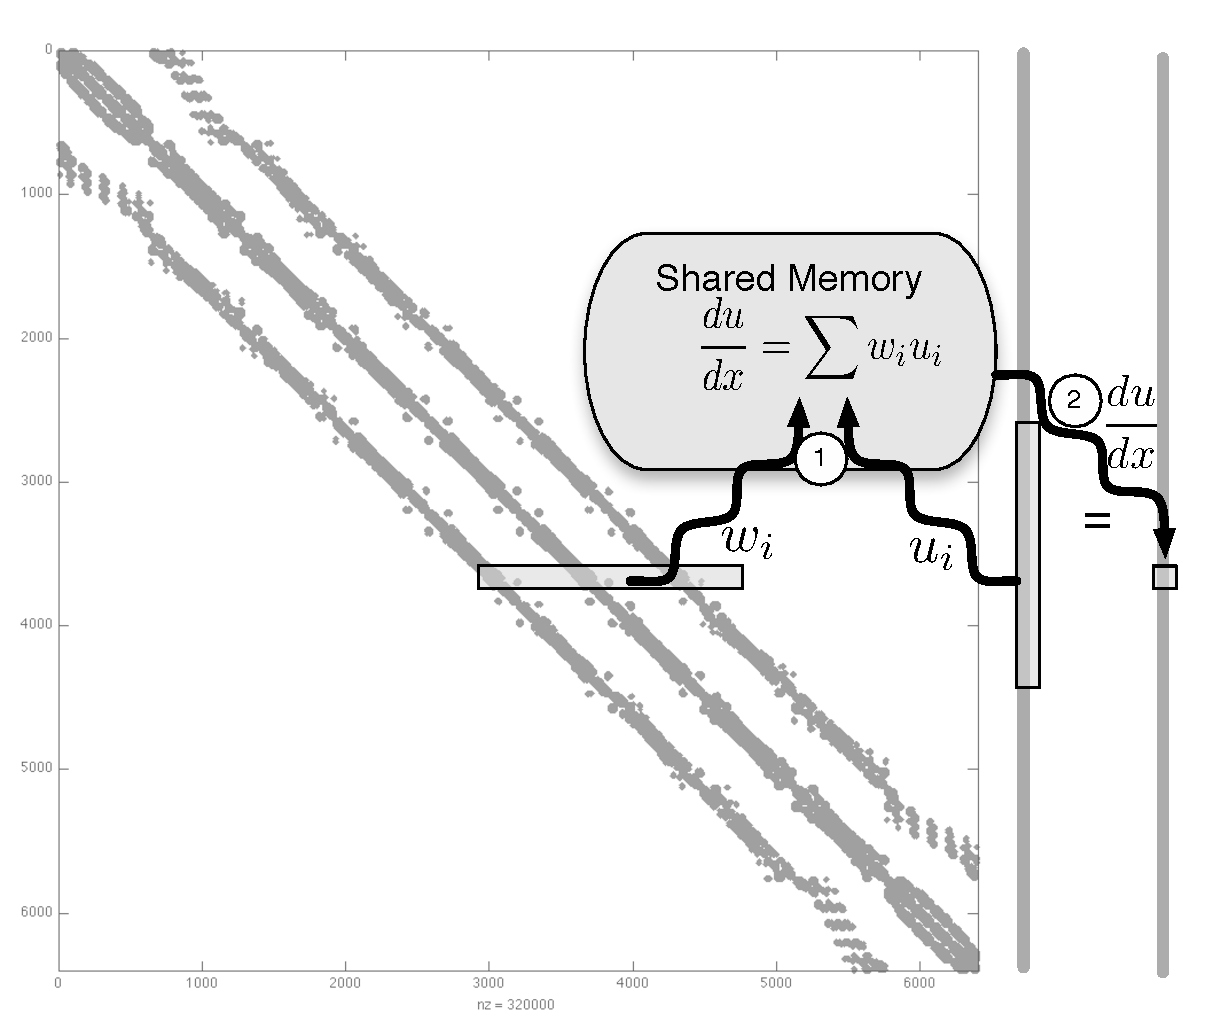
\includegraphics[width=3in]{figures/paper1/figures/omnigraffle/oneThreadPerStencil_GRAY.pdf}
      \caption{Naive approach to sparse matrix-vector multiply. Each thread is responsible for the sparse vector dot product of weights and solution values for derivatives at a single stencil.  }
      \label{fig:oneThreadPerStencil}
\end{figure}


\subsubsection{Alternate Approach: One warp per stencil} 

\begin{figure}[htbp]
      \centering
       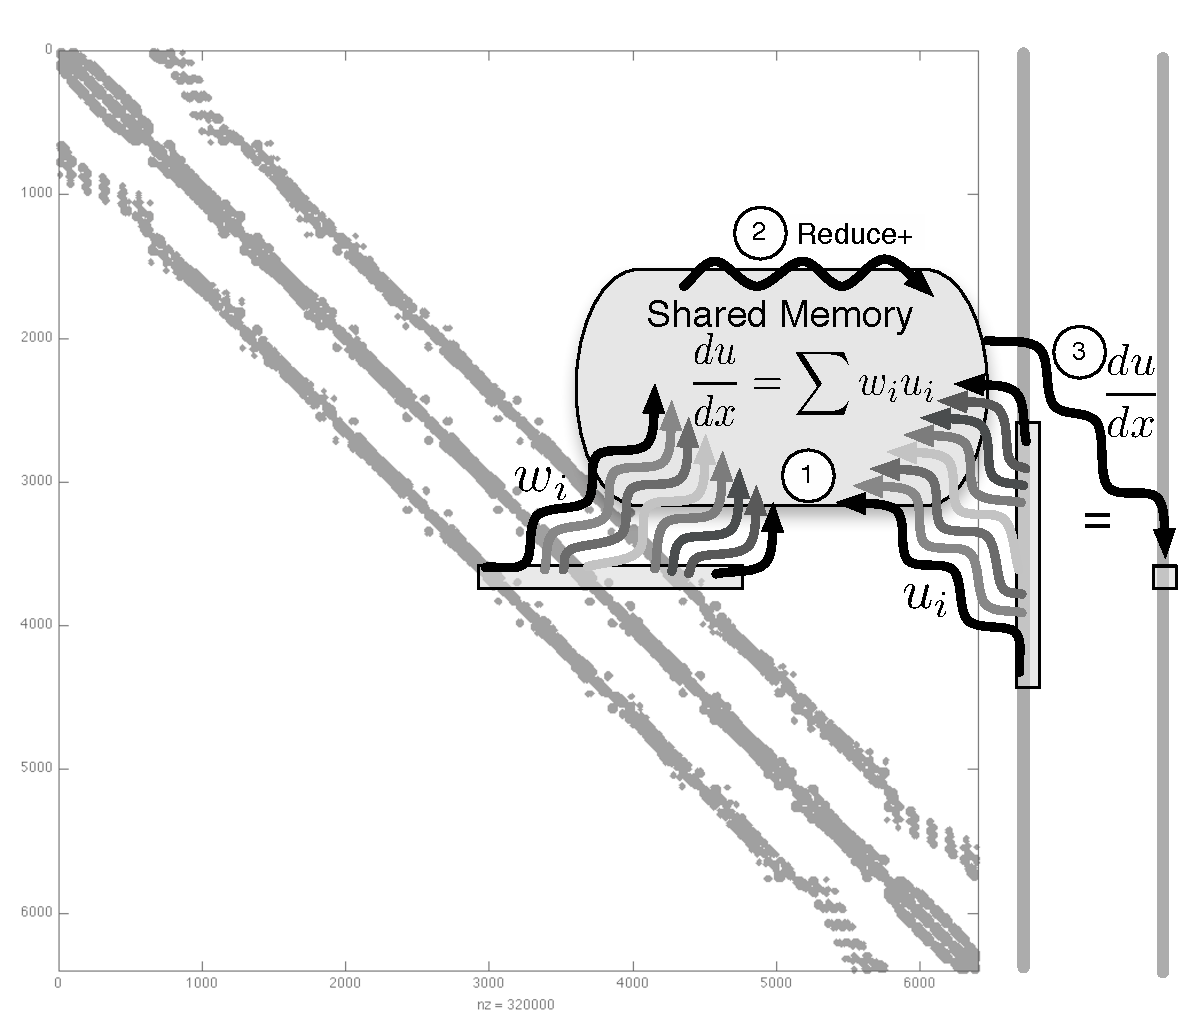
\includegraphics[width=3in]{figures/paper1/figures/omnigraffle/oneWarpPerStencil_GRAY.pdf}
      \caption{Alternative approach. A full warp (32 threads) collaborate to apply weights  and compute the derivative at a stencil center. }
      \label{fig:oneWarpPerStencil}
\end{figure}


An alternate approach, illustrated in Figure~\ref{fig:oneWarpPerStencil}, dedicates a full warp of threads to a single stencil. Here, 32 threads load the weights of a stencil and the corresponding elements of the solution vector. As the 32 threads each perform a subset of the dot product, their intermediate sums are accumulated in 32 elements of shared memory (one per thread).
Should  a stencil be larger than the warp size, the warp iterates over the stencil in increments of the warp size until the full dot product is complete. Finally, the first thread of the warp performs a sum reduction across the 32 (warp size)  intermediate sums stored in shared memory and writes the derivative value to global memory. 

By operating on a warp by warp basis, weights for a single stencil are loaded with a reduced number of memory accesses. Memory loads for the solution vector remain random access but see some benefit when solution values for a stencil are in a small neighborhood in the memory space. Proximity in memory can be controlled by node indexing (see e.g., \cite{Bollig2011} and \cite{Connor2009}). 

For stencil sizes smaller than 32, some threads in the warp always remain idle. Idle threads do not slow down the computation within a warp, but under-utilization of the GPU is not desirable. For small stencil sizes, caching on the Fermi can hide some of the cost of memory loads for the naive approach, with no idle threads, making it more efficient. The real strength of one warp per stencil is seen for large stencil sizes. 
As part of future work on optimization, we will consider a parallel reduction in shared memory, as well as assigning multiple stencils to a single warp for small  $n$. 


%\subsubsection{Boundary Conditions} 
%Boundary conditions are handled on the GPU in the following way: 

dirichlet: kernel copies dirichlet values into place \authnote{Need to dust off code}



\subsection{Fragments (integrate above)}


%The term \textit{General Purpose Computing on GPUs} (GPGPU) refers to the application of a Graphics Processing Unit (GPU) 
%to problems other than typical rendering tasks (i.e., vertex transformation, rasterization, etc). Driven by the gaming industry's 
%insatiable desire for more realistic graphics, GPU performance in the last decade years has grown tremendously compared to CPUs.

%Based on \cite{Jansen:2007, CudaGuide:2008, GTX280:2008, Core2Extreme:2008, FermiPrice:2009}, we see in Figure~
%\ref{fig:gpuevolution} the widening gap between compute capabilities on 
%the GPU and CPU. The latest GPUs are capable of approximately ten times the number of 
%floating point operations per second compared to the latest generation CPU. Naturally, this peak 
%performance comes with limitations: historically GPUs have always lagged behind the CPU in terms 
%of flexibility and programmability.

While the nomenclature used in this paper is typically associated with CUDA programming, the names \textit{thread} and \textit{warp} are used to clearly illustrate kernel execution in context of the NVidia specific hardware used in tests. OpenCL assumes a lowest common denominator of hardware capabilities to provide functional portability. However, intimate knowledge of hardware allows for better understanding of performance and optimization on a target architecture. For example, OpenCL assumes all target architectures are capable at some level of SIMD (Single Instruction Multiple Data) execution, but CUDA architectures allow for Single Instruction Multiple Thread (SIMT). SIMT is similar to traditional SIMD, but while SIMD immediately serializes on divergent operations, SIMT allows for a limited amount of divergence without serialization. 

At the hardware level, a \textit{thread} executes instructions on the GPU. On Fermi level GPUs, groups of 32 threads are referred to as \textit{warps}. A warp is the unit of threads executed concurrently on a single \textit{multi-processor}. 
In OpenCL (i.e., software), a collection of hardware threads performing the same instructions are referred to as a \textit{work-group} of \textit{work-items}. Work-groups execute as a collection of warps constrained to the same multiprocessor. Multiple work-groups of matching dimension are grouped into an \textit{NDRange}. The \textit{kernel} provides a master set of instructions
for all threads in an NDRange \cite{OpenCL2009}. 

%\authnote{Just rewrote this stuff directly in opencl terms}
%In software, a collection of threads is referred to as \textit{block}. In hardware, blocks exist as a collection of warps with the constraint that the entire collection executes on the same multiprocessor. Again in software, multiple 
%blocks of matching dimension are grouped into a \textit{grid}. The \textit{kernel} provides a master set of instructions
%for all threads in a grid, although each thread executes the instructions on different memory \cite{CudaGuide:2011}. 

%While the nomenclature used in this paper is typically associated with CUDA programming, the names \textit{thread} and \textit{warp} are used to clearly illustrate kernel execution in context of the NVidia specific hardware. OpenCL has one-to-one mappings for CUDA terminology at the software level, so the two can be used interchangeably. For example, OpenCL labels threads as \textit{work-items}. Blocks are \textit{work-groups}, and a grid is an \textit{NDRange} with an associated \textit{kernel} for an instruction set . 

NVidia GPUs have a tiered memory hierarchy related to the grouping of threads described above. 
In multiprocessors, each computing core executes a thread with a limited set of registers. The number of registers varies with the generation of hardware, but always come in small quantities (e.g., 32K shared by all threads of a multiprocessor on the Fermi). Accessing registers is free, but keeping data in registers requires an effort to maintain balance between kernel complexity and the number of threads per block. Threads of a single work-group can share information within a multiprocessor through \textit{shared memory}. With only 48 KB 
available per 
multiprocessor \cite{CudaGuide2011}, shared memory is another fast but limited resource on the GPU. OpenCL refers to shared memory as \textit{local memory}. 
Sharing information across multiprocessors is possible in \textit{global device memory}---the largest and slowest memory space on the GPU. To improve seek times into global memory, Fermi level architectures include L1 on each multiprocessor and a shared L2 cache for all multiprocessors.


%\textit{constant} and \textit{texture} memory caches are available for read-only access. 
%To use shared memory, 
%Threads must 
%explicitly copy intermediate computational results or data in and out. 

%Shared memory is divided evenly into 16 \textit{memory 
%banks} or 
%regions of memory that can be accessed simultaneously. Memory and registers can be accessed equally fast as long as no two 
%threads in the 
%same half-warp (i.e., first 16 threads or last 16 threads of the warp) are accessing the same memory bank. If this occurs, the 
%access is 
%considered to be a \textit{bank conflict} and the multiprocessor is forced to serialize memory access, increasing the delay until 
%the warp can 
%proceed with execution \cite{CudaGuide:2008}. 

%\begin{figure}[t] %  figure placement: here, top, bottom, or page
%   \centering
%   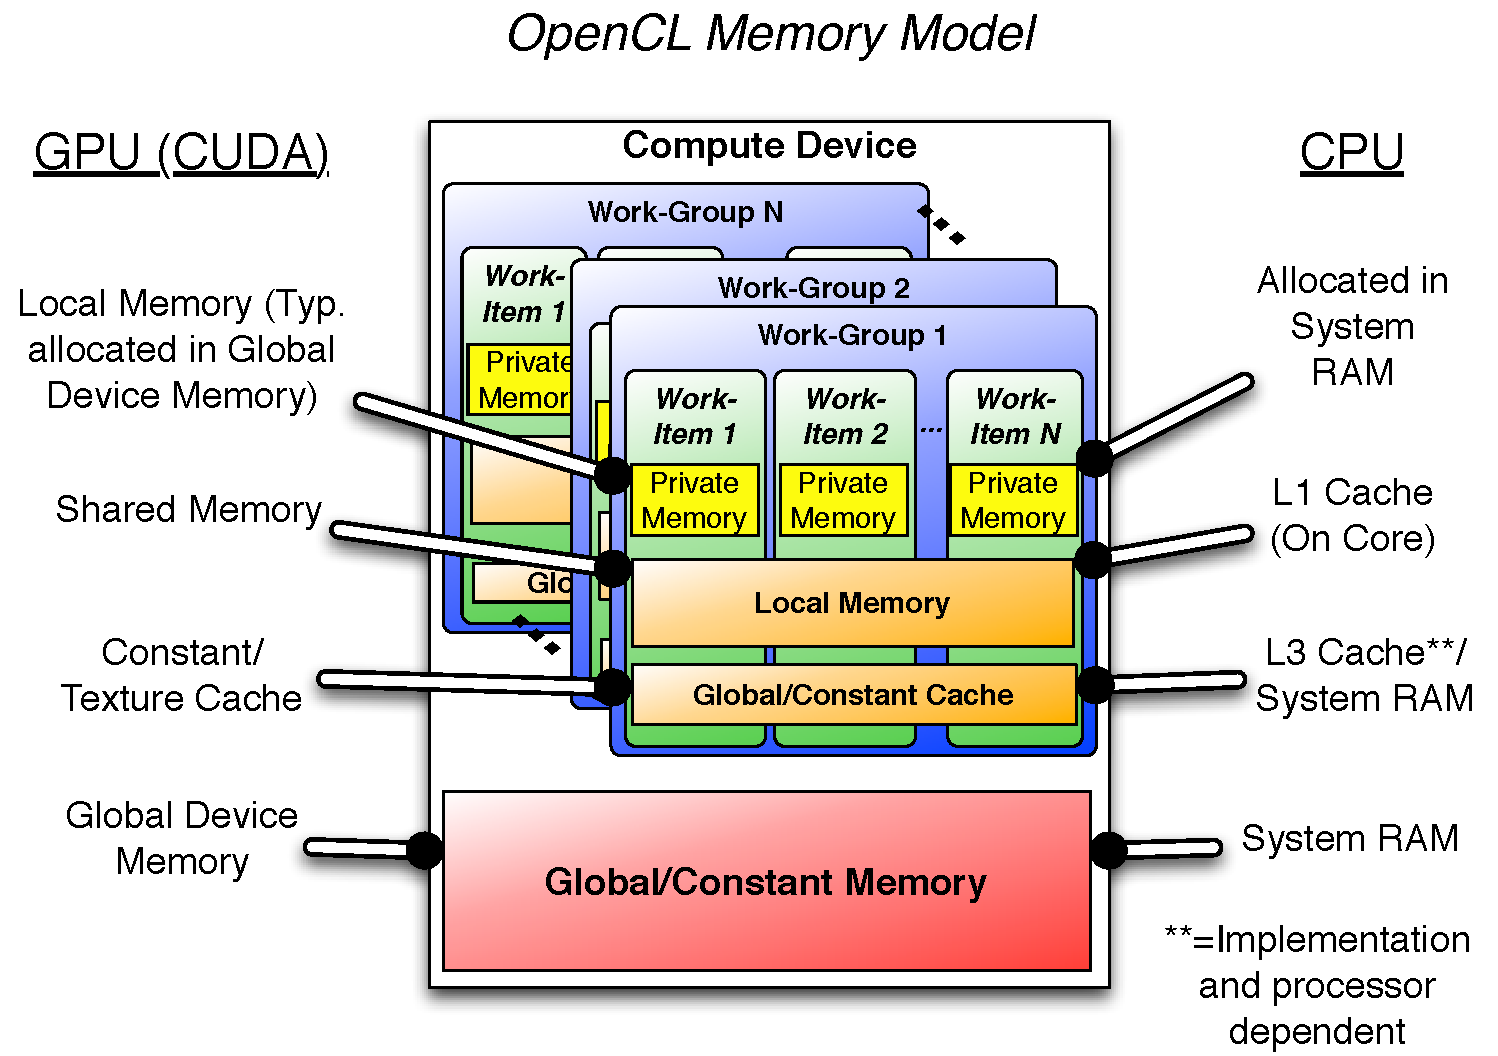
\includegraphics[width=4.5in]{figures/paper1/figures/opencl_memory_model.pdf} 
%   \caption{Comparison of GPU and CPU implementations underlying the OpenCL memory model for a single compute device.}
%   \label{fig:opencl_memory}
%\end{figure}
%


% and the place to which all data and kernels from the 
%CPU are copied for 
%execution. Note 
%that multiprocessors maintain read-only \textit{caches} for \textit{constants} and \textit{textures}---constants are values that 
%never change during kernel execution, 
%while textures are interpreted as read only arrays and provide a sophisticated cache mechanisms for certain types of non-sequential access. The real memory for constants and textures is part of the global device 
%memory, so reading 
%from texture and constant memory is faster than reads from global memory when no cache misses \cite{CudaGuide:2008}. 
%Also, if a kernel 
%uses too many registers per thread, \textit{local memory} is reserved in the global device memory to temporarily store register 
%contents for 
%later use with an associated penalty in efficiency \cite{CudaGuide:2008}. 

%Under OpenCL, the equivalent to CUDA local memory is called \textit{private memory} and is also reserved read-only per work-item in global device memory. CUDA's shared memory is labeled \textit{local memory} and shared by threads of a work-group. The CUDA texture and constant caches are known as \textit{Global/Constant Cache}, and similar to CUDA, exist outside of developer control. OpenCL refers to \textit{global memory} and \textit{constant memory} when referring to read/write and read-only sections of CUDA's global device memory (respectively). Finally, CUDA textures are equivalent to OpenCL \textit{buffers} (1D arrays) or \textit{images} (2D/3D arrays) \cite{OpenCL:2009}.

%Based on \cite{Behr:2009, OpenCL:2009}, Figure~\ref{fig:opencl_memory} compares the underlying implementation of the OpenCL memory hierarchy on GPUs and CPUs. Notably, on current CPUs most of the memory is reserved in System RAM, whereas the hierarchy naturally fits on the deep memory hierarchy of the GPU.  

\subsection{Implicit Solvers}

Perhaps this section should move up. I think it might be best to discuss GMRES and iterative methods before Distributed Solvers (that way we can say the general solution form is ``matrix form''. but in parallel we need to use distributed algorithms.